\let\negmedspace\undefined
\let\negthickspace\undefined
\documentclass[journal]{IEEEtran}
\usepackage[a5paper, margin=10mm, onecolumn]{geometry}
%\usepackage{lmodern} % Ensure lmodern is loaded for pdflatex
\usepackage{tfrupee} % Include tfrupee package

\setlength{\headheight}{1cm} % Set the height of the header box
\setlength{\headsep}{0mm}     % Set the distance between the header box and the top of the text

\usepackage{gvv-book}
\usepackage{gvv}
\usepackage{cite}
\usepackage{amsmath,amssymb,amsfonts,amsthm}
\usepackage{algorithmic}
\usepackage{graphicx}
\usepackage{textcomp}
\usepackage{xcolor}
\usepackage{txfonts}
\usepackage{listings}
\usepackage{enumitem}
\usepackage{mathtools}
\usepackage{gensymb}
\usepackage{comment}
\usepackage[breaklinks=true]{hyperref}
\usepackage{tkz-euclide} 
\usepackage{listings}
% \usepackage{gvv}                                        
\def\inputGnumericTable{}                                 
\usepackage[latin1]{inputenc}                                
\usepackage{color}                                            
\usepackage{array}                                            
\usepackage{longtable}                                       
\usepackage{calc}                                             
\usepackage{multirow}                                         
\usepackage{hhline}                                           
\usepackage{ifthen}                                           
\usepackage{lscape}

\begin{document}

\bibliographystyle{IEEEtran}
\vspace{3cm}

\title{4.6.3}
\author{EE25BTECH11015 - Bhoomika V}
% \maketitle
% \newpage
% \bigskip
{\let\newpage\relax\maketitle}

\renewcommand{\thefigure}{\theenumi}
\renewcommand{\thetable}{\theenumi}
\setlength{\intextsep}{10pt} % Space between text and floats


\numberwithin{equation}{enumi}
\numberwithin{figure}{enumi}
\renewcommand{\thetable}{\theenumi}
\parindent 0px 
{Question :-} 
Find the equation of the line which passes through the point $(-2,4,-5)$ and is parallel to the line
\[
\frac{x+3}{3} = \frac{y-4}{5} = \frac{z+8}{6}.
\]

\solution \\ 

Let the equation of line passing through the given point be
\[
\vec{x} = 
\begin{pmatrix}
-2 \\ 4 \\ -5
\end{pmatrix}
+ \mu \vec{d}
\]
where $\vec{d}$ is the direction vector of the line.  

The direction vector of the line 
\[
\vec{x} = 
\begin{pmatrix}
-3 \\ 4 \\ -8
\end{pmatrix}
+ \lambda
\begin{pmatrix}
3 \\ 5 \\ 6
\end{pmatrix}
\]
is
\[
\vec{d} = 
\begin{pmatrix}
3 \\ 5 \\ 6
\end{pmatrix}.
\tag{1}
\]

Thus, the required equation of the line is
\[
\vec{x} =
\begin{pmatrix}
-2 \\ 4 \\ -5
\end{pmatrix}
+ \mu 
\begin{pmatrix}
3 \\ 5 \\ 6
\end{pmatrix}.
\]
\begin{figure}[H]
\begin{center}
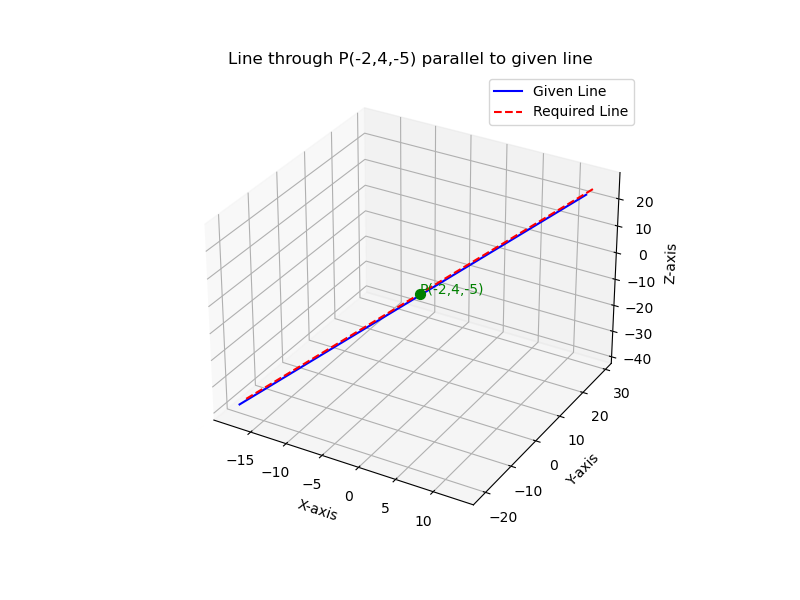
\includegraphics[width=0.6\columnwidth]{Figs/Fig1.png}
\end{center}
\caption{}
\label{fig:Fig.1}
\end{figure}

\end{document}
